\paragraph{tf.variable\_scope \& tf.name\_scope}

\paragraph{tf.sparse\_tensor}	tf中的稀疏张量。使用三个稠密的张量来表示。
\begin{itemize}
	\item indices: 表示原张量中非零值的位置
	\item values: 表示indices中元素所指位置上的值
	\item dense\_shape: 表示原张量的shape
\end{itemize}

\paragraph{defaultdict}python中的defaultdict,也是一种dict。与传统的dict不同,当传统的dict的key不存在时会Error,但defaultdict不会,而是返回一个默认值。该默认值由创建defaultdict时传入的参数有关:$dd = defaultdict(default_factory)$。

当default\_factory是list时,默认值是[],defaultdict其他常见取值还有:str, set, int, dict。但不可以是defaultdict。

\paragraph{glob}python中的一个内置模块,用于查找符合特定规则的文件路劲。如:
\begin{python}
	import glob
	pattern = "./myfloder/prefix-*.txt"
	li = glob.glob(pattern) # 此时li中就包含了所有符合pattern这个模式的文件名
\end{python}


\paragraph{np.argsort}对数组的元素进行排序(默认是从小到大),生成一个新的数组,数组元素是排序后的数组所对应的下标。
\begin{python}
	import numpy as np
	x = np.array([2,1,3,5,4])
	y = np.argsort(x) # y = [1, 0, 2, 4, 3]
	# 从大到小排序
	y = np.argsort(-x) # y = [3, 4, 2, 0, 1]
\end{python}
该方法还有更复杂的使用方法,可以根据参数进行调节,$argsort(a, axis=-1, kind=None, order=None)$。


\paragraph{tf.train.Saver}tf中用于保存、恢复模型参数的接口。主要由两个接口:1)tf.train.Saver().save()用于保存模型;2)tf.train.Saver().restore()用于回复模型。
\begin{python}
	import tensorflow as tf
	saver = tf.train.Saver(max\_to\_keep=3) # max\_to\_keep表示保存的checkpoint最大次数
	...
	# 保存模型
	# sess: 会话的名字
	# save\_path: 模型的保存路径
	# global\_step: 保存模型时的后缀
	# 使用以下方法保存模型后会产生四个文件,分别是:
	# checkpoint文件:会记录最新的模型是哪个
	# .ckpt.meta文件:包含元图,保存了计算图的结构,没有变量的值
	# .ckpt.data 文件:保存权重等参数
	# .ckpt.index 文件:为数据文件提供索引,{还不太确定}
	saver.save(sess=sess, save_path=model_save_path, global_step=step)
	...
	# 恢复模型
	# save_path可以不用加模型的后缀
	saver.restore(sess=sess, save_path=model_save_path)
\end{python}

\paragraph{tf.Session}运行tf中操作的类,Session类封装了运行操作所需要的环境。可以使用手动开启和关闭、上下文的方式使用Session。在使用Session时还可以进行配置,将配置作为Session初始化的参数传入。

\paragraph{tf中的RNN}RNN的训练数据与其他神经网络的训练数据有一点不一样。通常的NN中的训练数据,每个样本就是一个向量。但是在RNN中,每个训练样本就是一个矩阵,每一行表示一步的输入,正因为RNN所处理的问题不同,RNN的输出数据也变得更加复杂。\\
针对不同的RNN有不同形式的输出,但可以进行简单的归纳:对于RNN中的每个样本,其形式为$\mathbb{R}^{max\_time \times embed\_size}$,其中$max\_time$表示所有样本中序列的最大长度,$embed\_size$表示每一步的输入的长度。当输入了一个样本后,会将样本的每一行 --- 即每一步的数据输入到RNN中,由于RNN本身的特点,每一步都可以产生输出,通常来说包含每一步的输出和状态(具体到不同的RNN时会有不同)。每一步的输出维度会收到RNN模型隐层宽度 --- 即隐层单元数量的影响。并且针对不同的任务,最终需要的输出是不一样,例如m对n、m对1、m对m的任务等等。\\
在tf中,有多种关于RNN单元的类,如BasicLSTMCell、GRUCell、MultiRNNCell。可以在这些类的基础上搭建自己的RNN模型。

\paragraph{numpy设置随机数种子}$np.random.seed(seed)$。

\paragraph{C++数据类型转换}
\subparagraph{数字 <=> 字符串}
\begin{itemize}
	\item itoa: 整数转为字符串,可以设置基底
	\item stoi: 字符串转为整数 ,可以设置基底
	\item atoi、atol、atoll: 将字符串转为int/long/long long,可以设置基底
	\item to\_string: 可以讲数字转为字符串,包括整数、小数等
\end{itemize}

\paragraph{C++集合} 通过$\#include<set>$来引入set。关于集合的一些运算,包含在algorithm库中。在algorithm库中有一个includes函数,可以用来判断两个容器之间是否存在包含关系,但是,要注意\tbc{red}{两个容器都要先从小到大进行排序!!!}
\begin{cpp}
	// 省略头文件和库的包含代码
	int container[] = {5,10,15,20,25,30,35,45,50};
	int continent[] = {40,30,20,10};
	
	sort (container,container+10);
	sort (continent,continent+4);
	
	// using default comparison:
	if ( std::includes(container,container+10,continent,continent+3) )
		cout << "container includes continent!\n";
	else	cout<<"NO\n";
	
\end{cpp}


\paragraph{python format用法}
\subparagraph{对齐}"$\{:\}$" 通常将对齐符号放在$:$后。\^ 、| < | >分别是居中、左对齐、右对齐,在填充符号后面可带宽度,在$:$后可带填充字符,默认为空格。

\subparagraph{数字输出格式}主要包括小数位数(如.2f)、百分号输出(如.2\%)、指数形式输出(如.2e)、带正负符号的输出(如+.2f)、按不同进制的输出(b、d、o、x分别是二进制、十进制、八进制、十六进制,在b|o|x前加#可以输出进制符号,x的大小写会影响进制符号的大小写。
\begin{python}
	"{:^8}".format("居中")	# 居中显示,宽度为8,默认用空格填充
	"{:*<8}".format("左对齐")	# 左对齐显示,宽度为8,用*填充
	"{:*>8}".format("右对齐")	# 右对齐显示,宽度为8,默认用空格填充
	"{:.2f}".format(123)
	"{:.2%}".format(123)
	"{:b}".format(11)
	"{:d}".format(11)
	"{:o}".format(11)
	"{:x}".format(11)
	"{:#x}".format(11)
	"{:#X}".format(11)
\end{python}

\paragraph{numpy nan的处理}numpy中可以使用np.isnan()来判断数组中的元素是否为NAN,返回的结果与数组形状相同,元素为True/False,该位置的元素为NAN是则为True,否则为False。可以使用 np.nan\_to\_num(x, copy=True, nan=0, posinf= 1.7976931348623157e+308, neginf=-1.7976931348623157e+308) 来进行转换。该函数可以将NAN(包括无穷小、无穷大)转换为数字,可以指定转换后的数字。参数:x是待转换的数据,可以是数组或单个数字;copy表示是否进行原地转换,相当于pandas中的in\_place参数,但取值与in\_place相反;nan表示取代NAN的数字;posinf、neginf表示用什么取代正/负无穷。

\tbc{red}{找到数组中nan指的位置}:np.argwhere(np.isnan(a))。解释:通过np.isnan标记数组中nan值的位置为True,np.argwhere会返回那些True的下标。


\paragraph{matplotlib 中的marker}更多内容可参见:\href{https://matplotlib.org/api/_as_gen/matplotlib.pyplot.plot.html#matplotlib.pyplot.plot}{Matplotlib}
\begin{figure}[h]
	\centering
	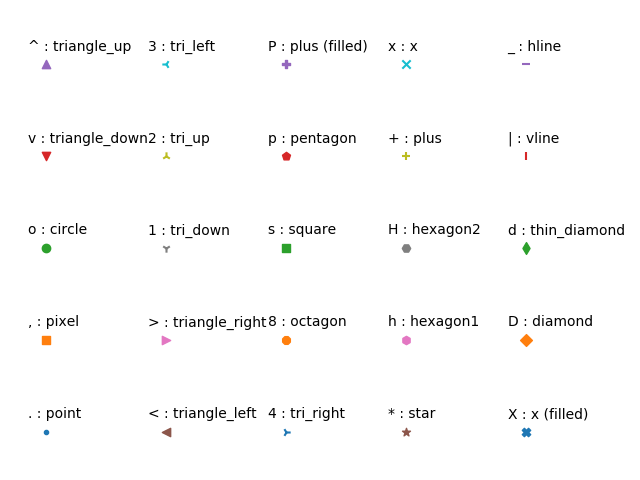
\includegraphics[width=.8\textwidth]{pics/markers.png}
	\caption{Matplotlib中的markers}
\end{figure}






